%%% Содержимое слайдов

% 1. Название, автор, руководитель.
% 2. Постановка задачи (актуальность)
% 3. способ (инструменты для) решения
% 4. результаты
% 5. анализ результатов
% 6. Заключение 

\frame[plain]{\titlepage} % Титульный слайд

%-------------------------------------------------------------------------------

\section{Постановка задачи}

\begin{frame}
\frametitle{\insertsection}

\begin{itemize}    
    \item Задачи электрокаротажа нелинейны, а обратная
    задача определения параметров по измерениям
    некорректна (неоднозначна). Решение задач в
    полных постановках весьма ресурсоемко и плохо
    подходит для промышленного применения

    \item На практике возникает необходимость в палетках с такими параметрами,
    которые не опубликованы. Поэтому была поставлена задача разработки метода
    решения прямой задачи БКЗ, которая позволила бы задавать необходимые
    параметры модели для построения палеток

    \item Решение краевой задачи в математической постановке прямой задачи БКЗ неэффективно уже имеющимися средствами
\end{itemize}
\end{frame}

%-------------------------------------------------------------------------------

\section{Способ решения}

\begin{frame}
\frametitle{\insertsection}

\textbf{Инструменты:}
\begin{itemize}
    \item Язык программирования Python c программными пакетами для паралелльных вычислений

    \item FEniCS — популярная вычислительная платформа с открытым исходным
    кодом (LGPLv3) для решения уравнений в частных производных (ДУЧП). Основано на методе конечных элеметнов, имеет интерфейс на Python

    \item Библиотека на Python triangle для триангуляции Делоне
    \item Компьютер: операционная система
    Ubuntu 18.04 LTS, процессор Intel Pentium 4415U 2.30 ГГц с 4 логическими
    процессорами
\end{itemize}
\end{frame}

%-------------------------------------------------------------------------------

\section{Результаты}

\begin{frame}
\frametitle{\insertsection}

\vspace{-0.5cm}
\begin{minipage}[t]{0.47\linewidth}
    \textbf{Модель 1}
    \center{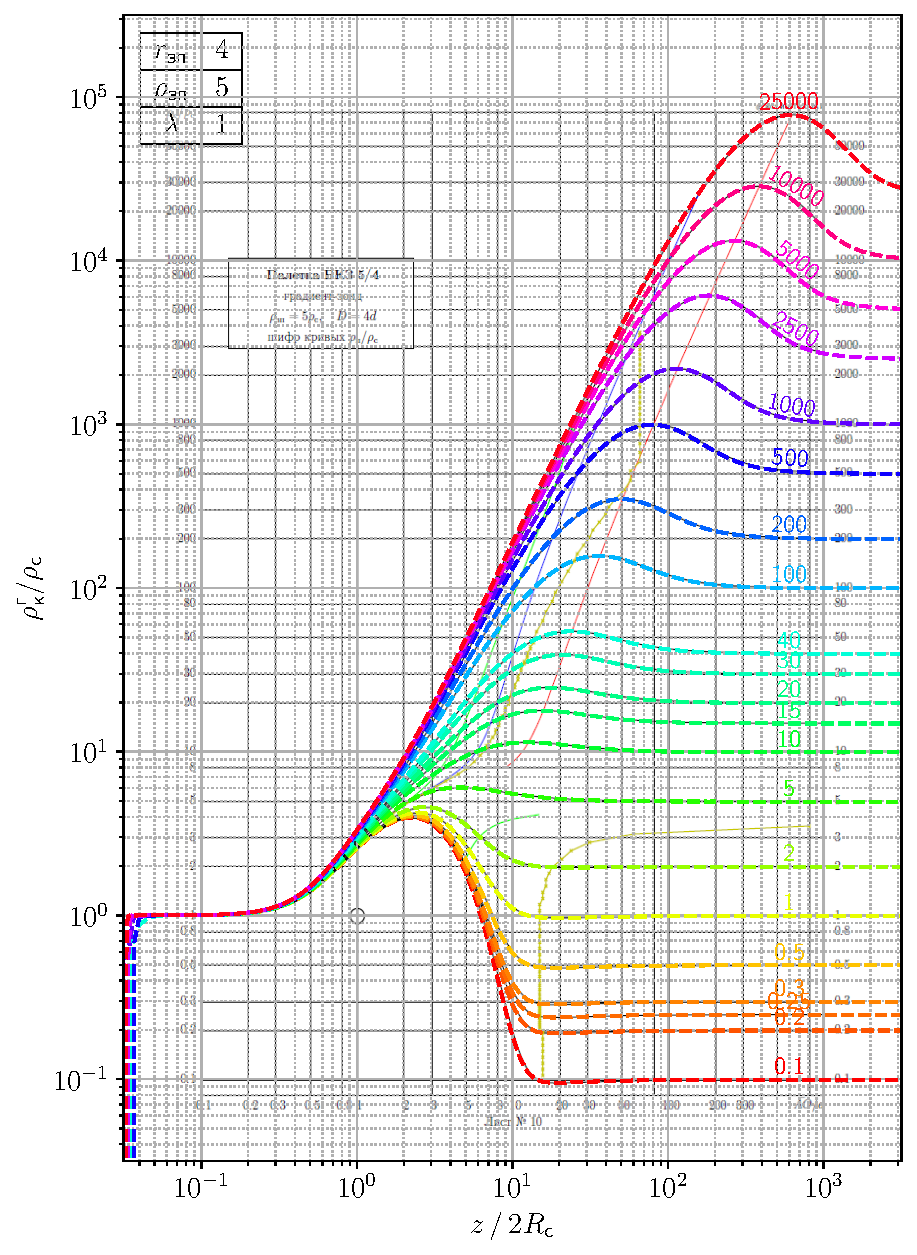
\includegraphics[width=1\linewidth]{plot_1_compare}}
\end{minipage}
\hfill
\begin{minipage}[t]{0.47\linewidth}
    \textbf{Модель 2}
    \center{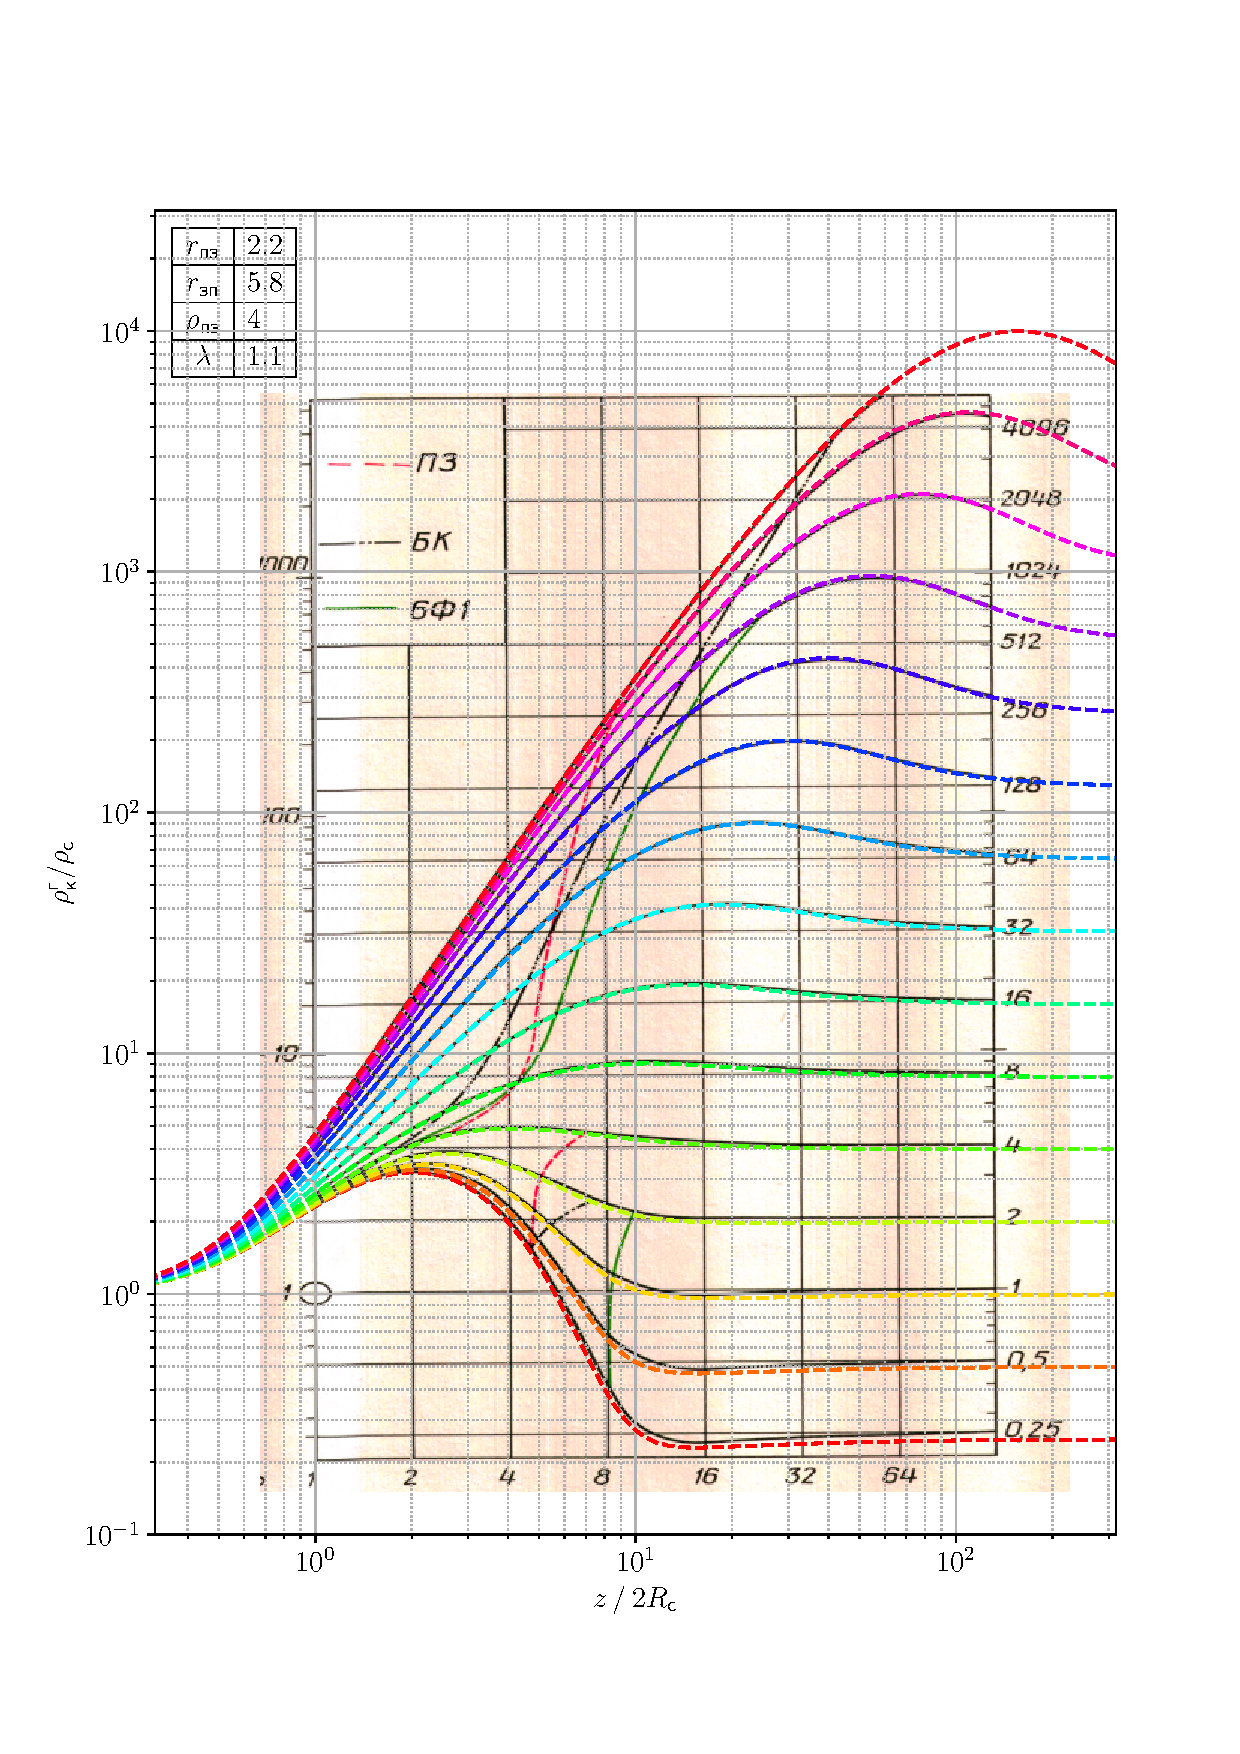
\includegraphics[width=1\linewidth]{plot_2_compare}}
\end{minipage}

\end{frame}

%-------------------------------------------------------------------------------

\section{Анализ результатов}

\begin{frame}
\frametitle{\insertsection}

\textbf{Модель 1:}
\begin{itemize}
    \item Время вычисления расчетной палетки ${18 \text{ c } \pm 159 \text{ мс }}$, 7 проходов
\end{itemize}

\textbf{Модель 2:}
\begin{itemize}
    \item Время вычисления расчетной палетки ${16.5 \text{ c } \pm 176 \text{ мс}}$, 7 проходов
\end{itemize}

Наблюдается совпадение, означает, что способ решения верный и точный

\end{frame}

%-------------------------------------------------------------------------------

\section{Заключение}

\begin{frame}
\frametitle{\insertsection}

\begin{itemize}
    \item Освоены пакеты программ для параллельных вычислений: вычислительная платформа для автоматического решения ДУЧП FEniCS, библиотека Python для векторных вычислений Numpy
    \item Проведены расчеты и сопоставление с известными результатами в литературе
    \item Показана применимость метода решения прямой задачи БКЗ с приемлимой точностью
    \item Все вычисления произведены на компьютере: операционная система
    Ubuntu 18.04 LTS, процессор Intel Pentium 4415U 2.30 ГГц с 4 логическими
    процессорами (1 физический процессор × 2 ядра в физическом процессоре ×
    2 потока в каждом ядре)
\end{itemize}

\end{frame}

%-------------------------------------------------------------------------------
